% Slide: What is Kunai?
\begin{frame}
	\frametitle{Kunai: what is it?}

	% Content: High-level introduction to Kunai, its purpose, and how it compares to Sysmon.
	\textbf{Kunai}\footnote{\url{https://github.com/kunai-project}} is a security monitoring tool focusing on \textbf{threat detection} and \textbf{threat hunting tasks}. For those familiar with \textbf{Microsoft Sysmon}\footnote{https://learn.microsoft.com/en-us/sysinternals/downloads/sysmon} you can view \textbf{Kunai} as its alter-ego for \textbf{Linux} systems.

	\vspace{1em}

	\par
	It allows the monitoring of several system-related events:
	\begin{itemize}
		\item binary / script execution
		\item shared objects loaded
		\item drivers loaded
		\item eBPF programs loaded
		\item \ldots
	\end{itemize}

	\par
	\vspace{1em}
	List of \textbf{events}: \url{https://why.kunai.rocks/docs/events/}
\end{frame}

% Slide: Execve Event Example
\begin{frame}
	\frametitle{Example: execve event}

	% Content: Visual example of an execve event with a note about elided fields.
	\centering
	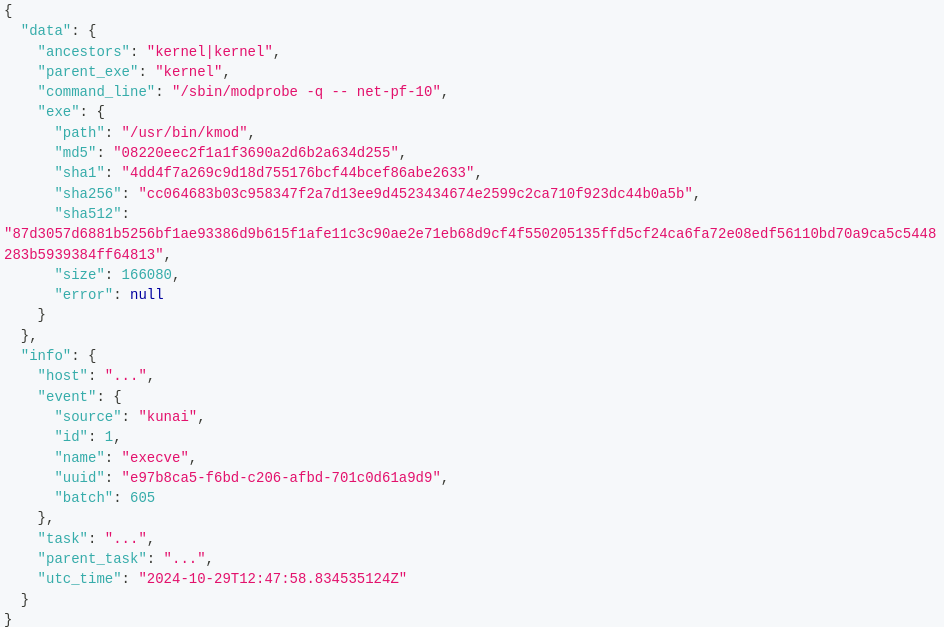
\includegraphics[width=0.9\textwidth]{img/kunai-execve.png}

	\textbf{NB:} parts with \textbf{"\ldots"} are elided for sake of space, please read documentation to understand the full event format.
\end{frame}

% Slide: Binary Analysis with Kunai
\begin{frame}
	\frametitle{How can it be used for binary analysis?}

	% Content: Explanation of how Kunai can assist with binary analysis despite not being its primary purpose.
	\textbf{Spoiler alert}: the primary goal of \textbf{Kunai} is not to be a binary analysis tool. Therefore it does not contain any advanced anti-analysis countermeasure some malware may implement.

	\vspace{1em}
	\par
	Yet we believe it can be useful to achieve the following:
	\begin{itemize}
		\item Get a quick overview of the capacities of a malware sample
		\item It is monitoring \textbf{system-wide} events, so it catches some execution indirections:
		      \begin{itemize}
			      \item cronjobs
			      \item services
			      \item dynamic linker tricks (example: LD\_PRELOAD trick)
			      \item \ldots
		      \end{itemize}
		\item \textbf{Kunai output} can be directly \textbf{shared}, \textbf{used} as \textbf{IoC}, or to create \textbf{detection rules}.
	\end{itemize}
\end{frame}

% Slide: Analysis Process in Theory
\begin{frame}
	\frametitle{Analysis process, in theory}

	% Content: Step-by-step process for analyzing malware using Kunai.
	\begin{enumerate}
		\item Run \textbf{Kunai} on a machine dedicated to \textbf{dynamic malware analysis} (ideally a Virtual Machine).
		\item Run the malware sample you want to look at.
		\item Let the malware run for some time so that you can capture the maximum of its activity.
		\item Collect the \textbf{Kunai} traces and analyze them.
		\item \textbf{Optional}: build \textbf{detection rules}\footnote{\url{https://why.kunai.rocks/docs/advanced/rule_configuration#detection-rules}}, extract \textbf{IoCs}, and share them.
	\end{enumerate}
\end{frame}

% Slide: Analysis Process in Practice
\begin{frame}
	\frametitle{Analysis process in practice}

	% Content: Highlight the Kunai sandbox project and its benefits for analysis automation.
	Use our \textbf{Kunai sandbox} project: \url{https://github.com/kunai-project/sandbox}

	\vspace{1em}

	\begin{itemize}
		\item It automates the procedure explained in the previous slide.
		\item It can be used to analyze samples from different architectures (currently \textbf{x86\_64} and \textbf{amd64}) $\rightarrow$ can be used to analyze \textbf{IoT and mobile devices} malware.
	\end{itemize}
\end{frame}

% Slide: Example Analysis - Mirai
\begin{frame}
	\frametitle{Example: Mirai}

	% Content: Showcase a real-world example of Kunai's output, highlighting its capability.
	Malware activity graph built from \textbf{Kunai} logs:
	\begin{center}
		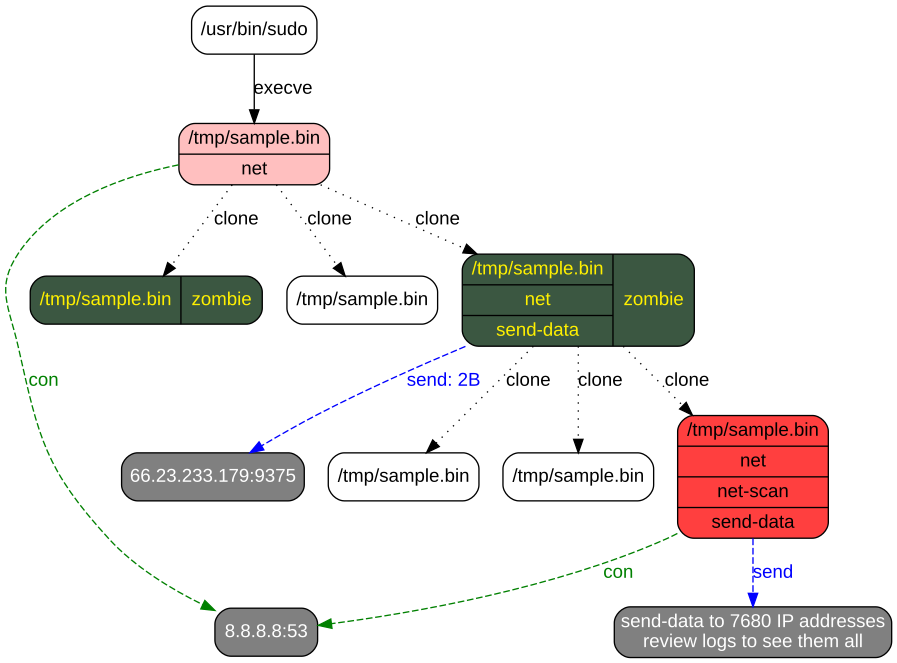
\includegraphics[width=0.8\textwidth]{img/kunai-sample.png}
	\end{center}
\end{frame}

% Slide: Going Further
\begin{frame}
	\frametitle{Going Further}

	% Content: Provide resources for learning, contributing, and further engagement with Kunai.
	\begin{itemize}
		\item Read the documentation: \url{https://why.kunai.rocks/}
		\item Do hands-on exercises: \url{https://github.com/kunai-project/workshops}
		\item Check out some malware traces: \url{https://helga.circl.lu/NGSOTI/malware-dataset}
		\item Contribute:
		      \begin{itemize}
			      \item Join the Discord channel.
			      \item Open issues for bugs, feature requests, \ldots
			      \item Give feedback: what you like and what you don't like.
		      \end{itemize}
	\end{itemize}
\end{frame}
